\chapter{Sensor nodes}
\label{chap:nodes}

This chapter will describe functionalities of sensor node devices. After that it will describe how electronic parts were chosen. A separate section will include details regarding \ac{PCB} design while another section will follow the production from first prototype to the production. Finally, it will be shown how the board is installed and integrated into the system.

\section{Physical design and connections}

Most of the required \ac{PCB} features were already described in the previous chapter - board should allow direct connection of \ac{FSR} sensors, it should eliminate need for additional perforated boards and it should provide a more robust solution for physical board position detection. Furthermore, it should feature low power consumption and enable connection of at least two rows of 8 pressure sensors. Also it should feature small dimensions because and provide mounting holes so that it doesn't have to be suspended by wires or be taped to the bed. The ideal position for the installation of the board is under the bed base slates. This way it can easily be serviced.

There are 4 variants of pin endings found on \ac{FSR} sensors. A variant with no leads is used for custom pin endings while solder tabs variant is used for direct soldering to the board. Because of the materials used for construction of the sensor, when heat is applied using standard soldering iron, there is a high possibility of sensor leads melting. This is why a female plug connector option was chosen. Distance between leads is $1/10"$ and they are compatible with standard \ac{PCB}connector pins. Since sensors will be mounted on pressure disks which are found on the upper side of the bed base, while the board is found under the slates, elongation cables are required. In this case, DuPont "jumper" cables will be used and a board connectors have been designed in such a way. Two edges of the board, are populated with 8 two-row connectors. Row on the top is connected to the \ac{ADC} pins of the microcontroller while the bottom pins are grounded. In front of each of the pin, a reference resistor $R_ref$ is found.

Connector that was used for internal communication bus features 6 wires - 2 wires are used for \ac{I2C}, 2 are used for power supply and 2 are used for physical position recognition. Because they are interchangeable with DuPont jumper wires and because of toolless cable connector installation, \ac{IDC} cables and connectors were used\cite{IDC}. There are two 3x2 internal communication bus connectors on the board so that boards can easily be "daisy-chained". Close to the first connector, two pull-down resistors for I2C bus are situated. For microcontroller programming, the same type of connectors was used. The cortex debug interface consists of 10 pins so a single 5x2 connector was used. Graphic \ref{fig:connectors} shows connectors with positions of pins.

\begin{figure}[h]
  \begin{center}
    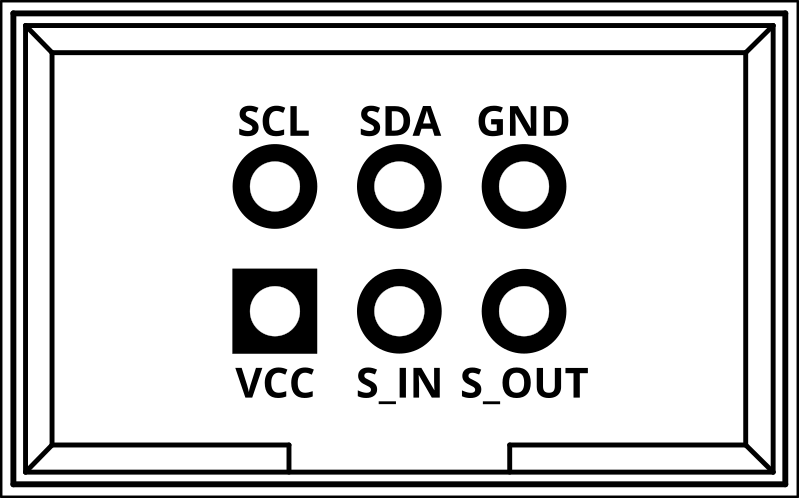
\includegraphics[height=2cm]{2-internal_bus.png}
    \hspace{1cm}
    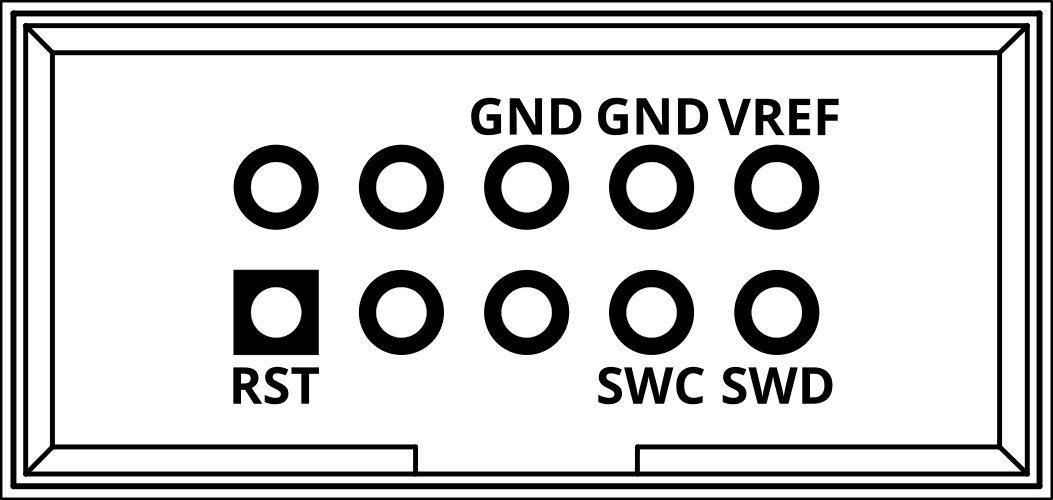
\includegraphics[height=2cm]{2-cortex_debug.png}
  \end{center}
  \caption{Internal communication bus and programming connector layout.}
  \label{fig:connectors}
\end{figure}


To power the microcontroller and because of debugging possibilities, a type B micro \ac{USB} connector was also added to the board. \ac{USB} connection features 2 differential data signals, a $5V$ and ground. Connector additionally has a "on-the-go" identification pin which is left floating because the requirement does not require a board to become \ac{USB} host. What board implements is a PRTR5V0U2X \ac{ESD} diode\cite{PRTR} which helps protect both the host \ac{PC} and the \ac{PCB} from electrical stress in form of surge or overvoltage.


\section{Component selection and compatibility}

A most important part of the node circuit is a microcontroller. Main requirement for it was the possibility of connecting 16 \ac{ADC} devices without the use of additional \ac{ADC} \ac{IC}s. Since other members of \ac{UC-Lab} have experience with programming Atmel microcontrollers, a choice was between ATxmega 8-bit AVR microcontrollers, 32-bit UC3 AVR microcontrollers and Atmel SMART ARM-based \ac{MCU}s\footnote{(abbrev. SAM)}. So let's take a look at a sample microcontroller from each of the categories. \textit{ATxmega64C3} is a 8-bit AVR microcontroller which features 64KB flash program storage and 4KB of \ac{RAM}, 16 pins provide \ac{ADC} with 12-bit resolution and there is native support for I2C\cite{ATxmega32C3}. \textit{AT32UC3C164C} is a 32-bit AVR microcontroller with the same flash size and number of 12-bit \ac{ADC} inputs but it features 20KB \ac{RAM}\cite{AT32uc3}. ATSAMD21J16 is a 32-bit ARM based microcontroller which has 8KB \ac{RAM}, 20 \ac{ADC} channels which have programmable gain stage, automatic offset and gain compensation as well as a possibility to oversample the signal to get 16-bit resolution\cite{ATSAMD}. Considering that this microcontroller is cheaper than both AVR microcontrollers and that it supported by multiple third-party frameworks such as ARM mbed, Arduino and Simba, Atmel SAMD was chosen as a microcontroller family that will be used. Atmel SAMD \ac{MCU} family microcontrollers have a naming pattern which makes easy to distinguish chips characteristics. An example will be described on is SAMD21J16B-AU. \textit{SAMD} is product family, \textit{21} is product series, \textit{J} stands for pin count (j = 64pins), \textit{16} is for flash memory density (16 = 64KB), \textit{B} is chip variant, \textit{A} is for package type (a = \ac{TQFP}) and finally \textit{U} is for package grade (U = -40 - 85$^{\circ}$C). A first prototype of the board was developed using \textit{ATSAMD21J18-AU} which is the same as one found in Atmels \textit{SAM D21 Xplained Pro Evaluation Kit} but that processors was out of stock when production boards were to be made. This is why \textit{ATSAMD21J16-AU}, a pin-compatible variant with 64KB instead of 256KB of RAM, was used in production boards. Pin layout of a \ac{TQFP} package can be seen in Figure \ref{fig:pinout}. This pinout is same for all ATSAMD21 microcontrollers with 64-pin \ac{TQFP} package so even smaller memory versions can be used for the cost-saving. 

\begin{figure}[h]
  \begin{center}
    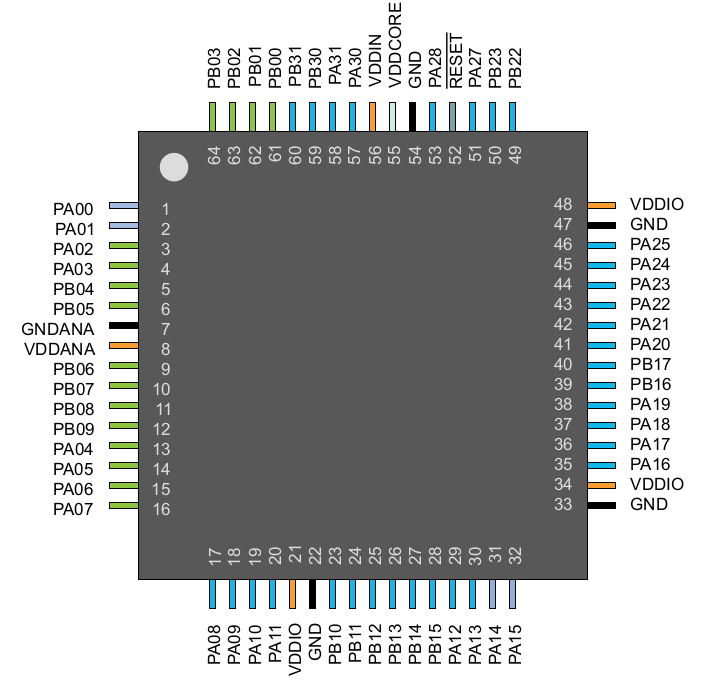
\includegraphics[width=0.4\linewidth]{2-pinout.png}
  \end{center}
  \caption{AT SAMD 64-pin TQFP package pin layout.}
  \label{fig:pinout}
\end{figure}

To power the selected microcontroller a $3.3V$ source is used. Since the most important feature the microcontroller does is analog to digital conversion, it's very important to have a stable and ripple-free \ac{DC} power supply. Oscillations in input voltage to the microcontroller may lead to inconsistent voltage readings. \ac{SMPS} is a very efficient way of \ac{DC}-\ac{DC} conversion but it suffers from a constant high and low frequency voltage ripple. Most of high frequency and some of low frequency ripple can be countered by using ferrite beads and capacitors but ripple still remains. Breakout board for Intel Edison, an endpoint used in this project, uses TPS62133 $5V$ step-down \ac{SMPS} which can supply a maximum of $3A$ of current\cite{edison_breakout}\cite{TPS6213}. Out of available $15W$, Intel Edison consumes on average $0.41W$ with Wi-Fi enabled. This means that it is possible to use the same power supply for powering the nodes. To filter out the noise a \ac{LDO} is found on each of the nodes. This is in accordance to the specification for high-performance \ac{ADC} power supply design provided by Texas Instruments\cite{SMPS}. \ac{LDO} that was chosen for this project is LD1117 which provides a stable $3.3V$ power supply with $1.1V$ dropout voltage. Input and output voltage lines of the power supply are bridged to the ground with capacitors to filter out the input noise. For debugging a $3.3V$ source can be attached to ${VREF}$ pin of the programming connector.


\section{PCB design and production}

A \ac{PCB} was designed in KiCad open-source tool for electronics design automation. First a microcontroller was placed with decoupling capacitors and ferrite bead according to the manual\cite{ATSAMD}. This ensures low noise during operation. After already described internal bus, programming, sensor connection and  micro USB connectors were placed, \ac{PCB} was populated with 2 status \ac{LED}s. First \ac{LED} serves as on/off detection and is directly connected to the $V_{cc}$ while the other one is user programmable and can be used for debugging. Board also has a power supply and a reset button. On 3 edges of the board a $3mm$ diameter holes were placed for easy mounting. The layout of the \ac{PCB} can be seen in Figure \ref{fig:pcb_kicad}.

\begin{figure}[h]
  \begin{center}
    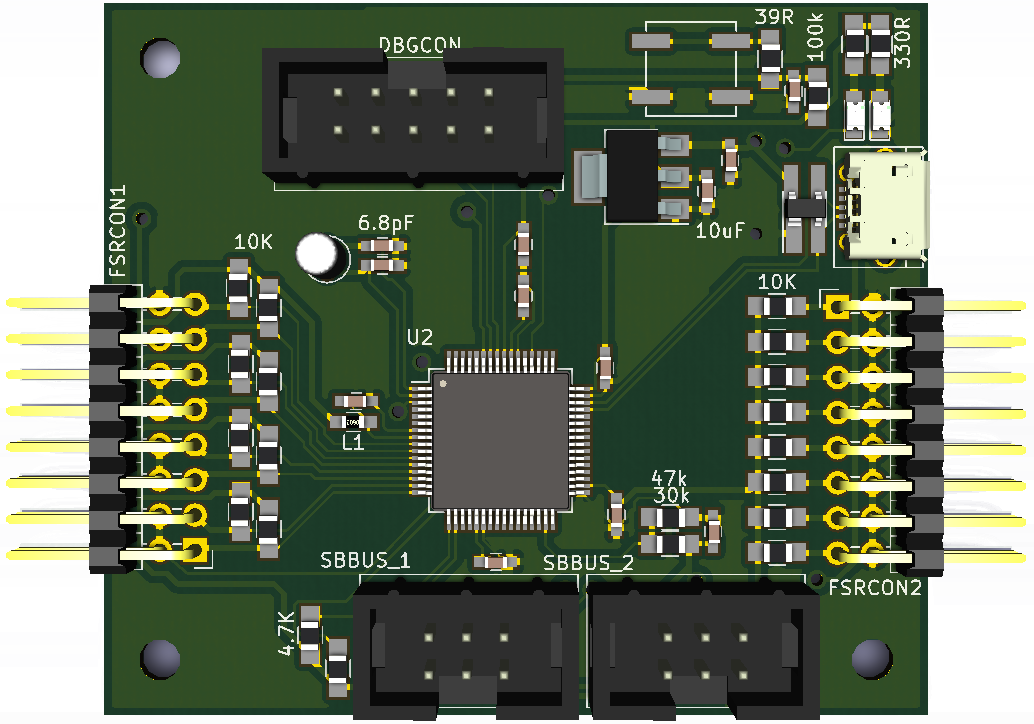
\includegraphics[width=0.45\linewidth]{2-pcb_kicad.png}
    \hspace{1cm}
    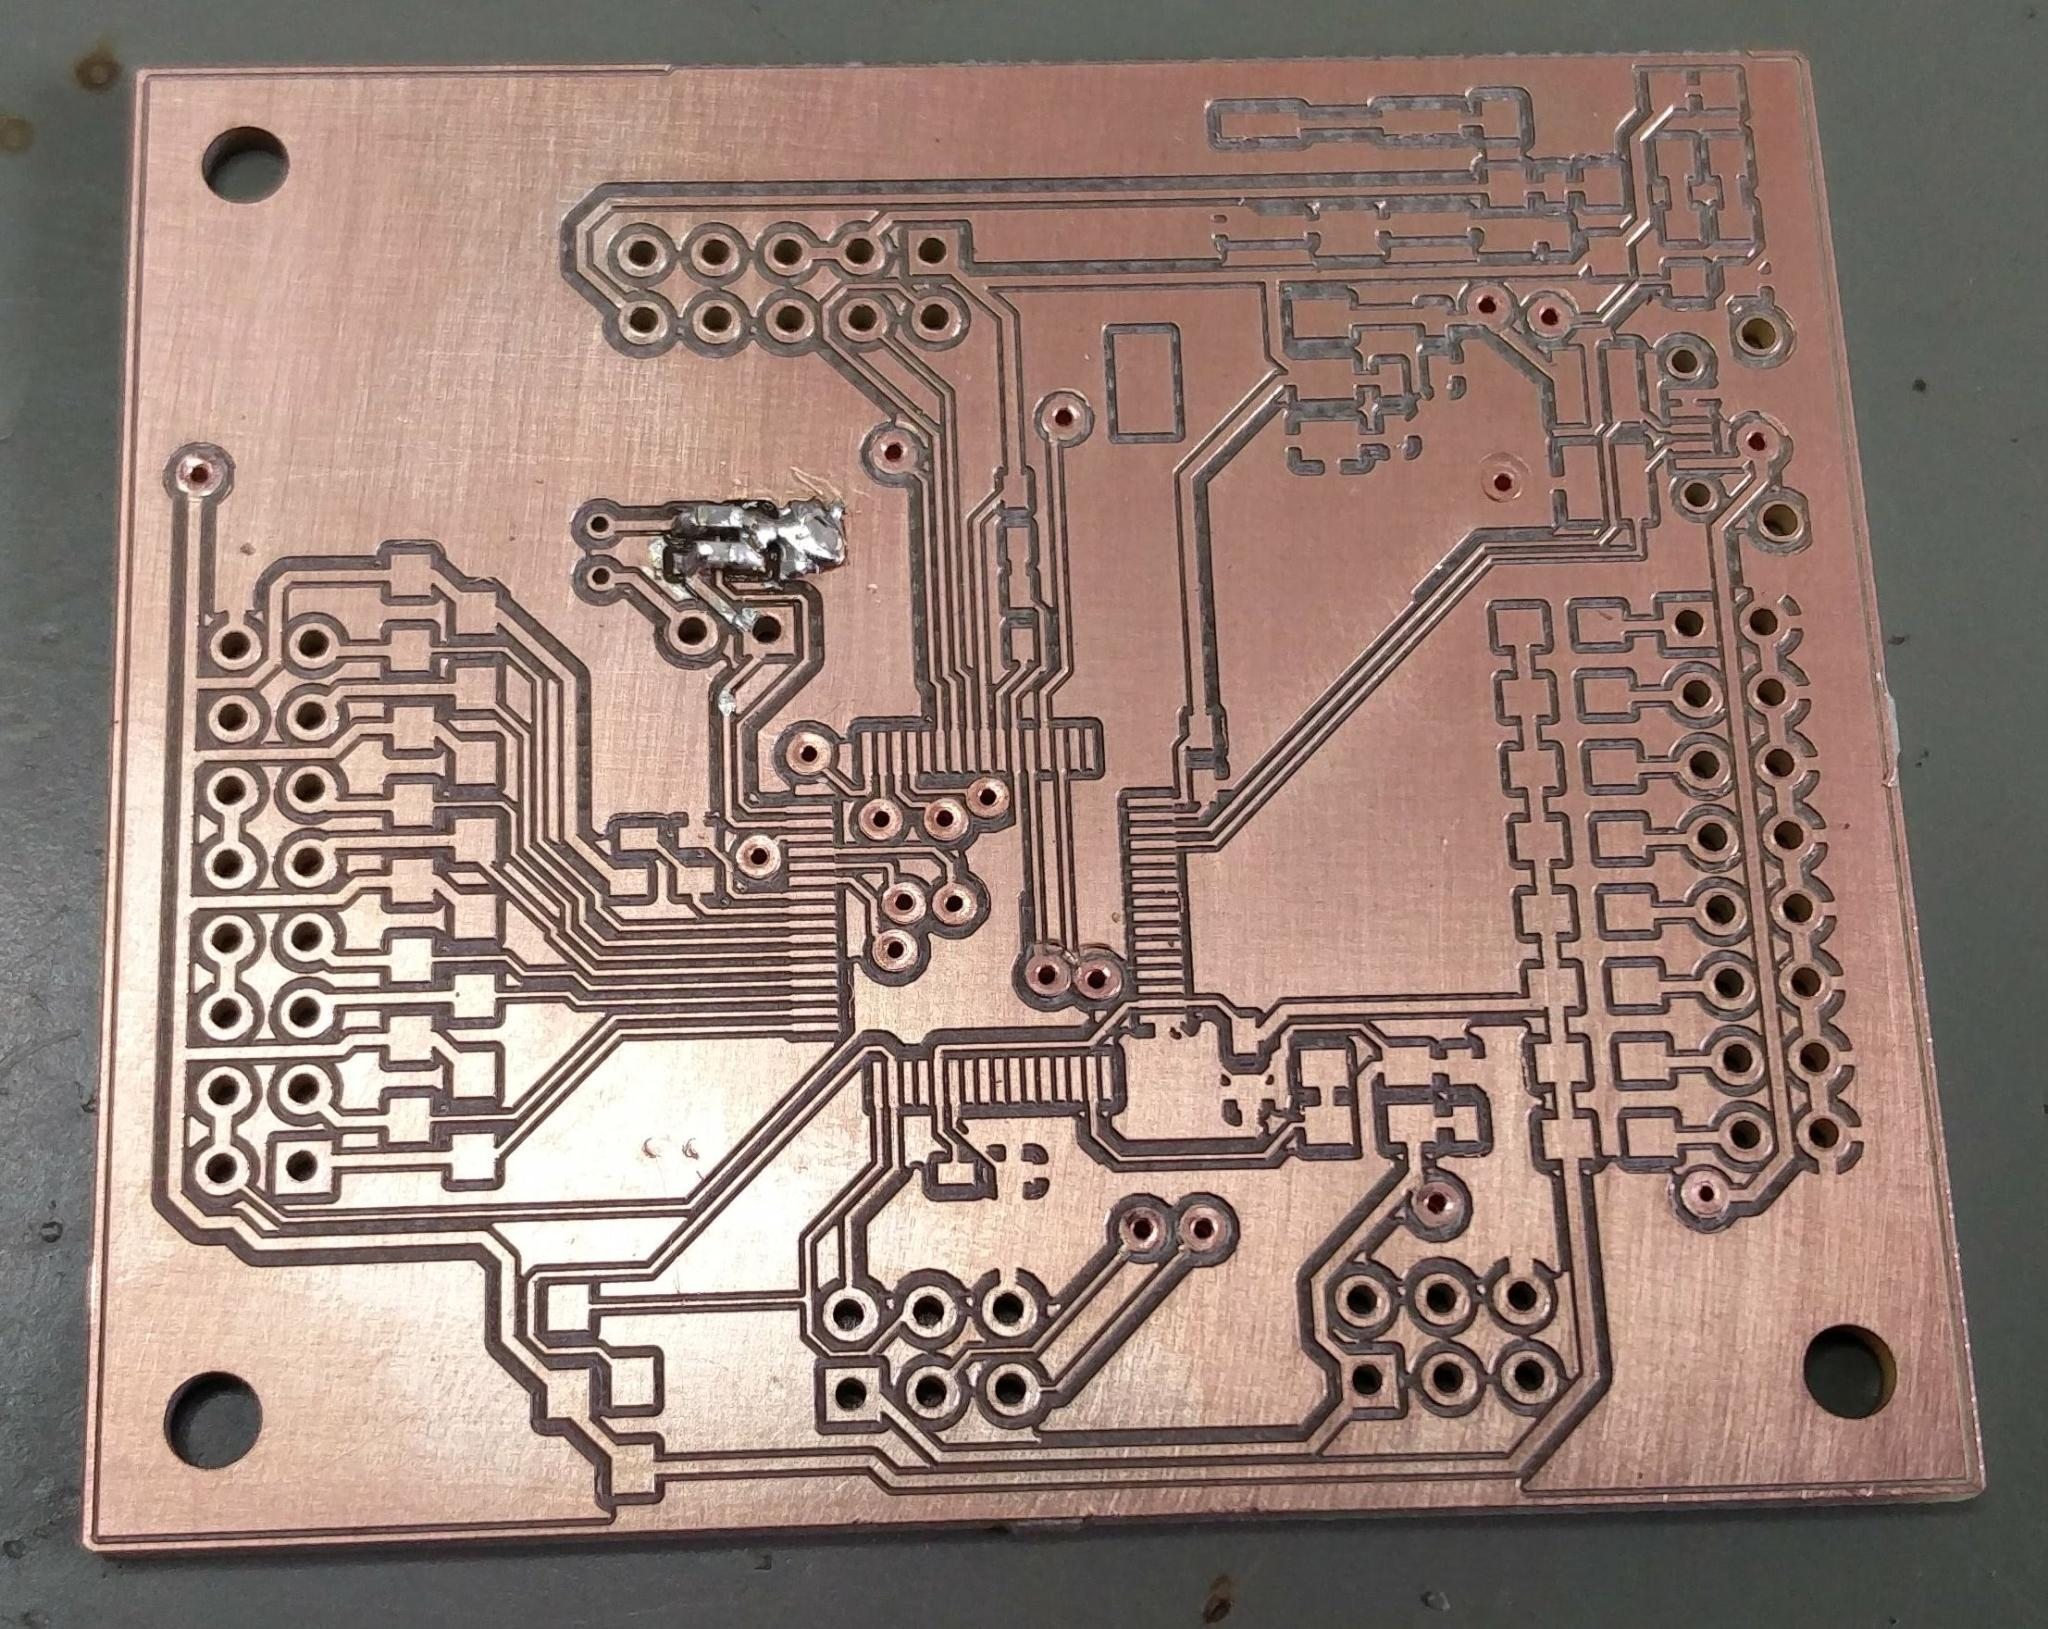
\includegraphics[width=0.4\linewidth]{2-pcb_milled.jpg}
  \end{center}
  \caption{3D view and prototype of printed circuitboard developed for the project.}
  \label{fig:pcb_kicad}
\end{figure}

To test the initial design, a board was milled at Department of Electronics at \ac{HTWG} using \href{http://www.lpkf.com/products/rapid-pcb-prototyping/circuit-board-plotter/protomat-s63.htm}{LPKF ProtoMat S63 circuit board plotter}. Since board design features vias, they had to be filled with copper rivets. Prototype production showed that micro USB pin had switched GND and USB OTG ID pins. This error happened due to difference of pin naming between footprint and schematic during the design. After this issue was fixed a board was sent for production to \href{https://aisler.net/}{AISLER}. The components were ordered from DigiKey with already described change from ATSAMD21J18 to ATSAMD21J16. 3 boards were produced and were hand soldered. After production, every board was tested with a sample program reading from each of sensors. The final and assembled board can be seen in Figure \ref{fig:pcb_production}

\begin{figure}[h]
  \begin{center}
    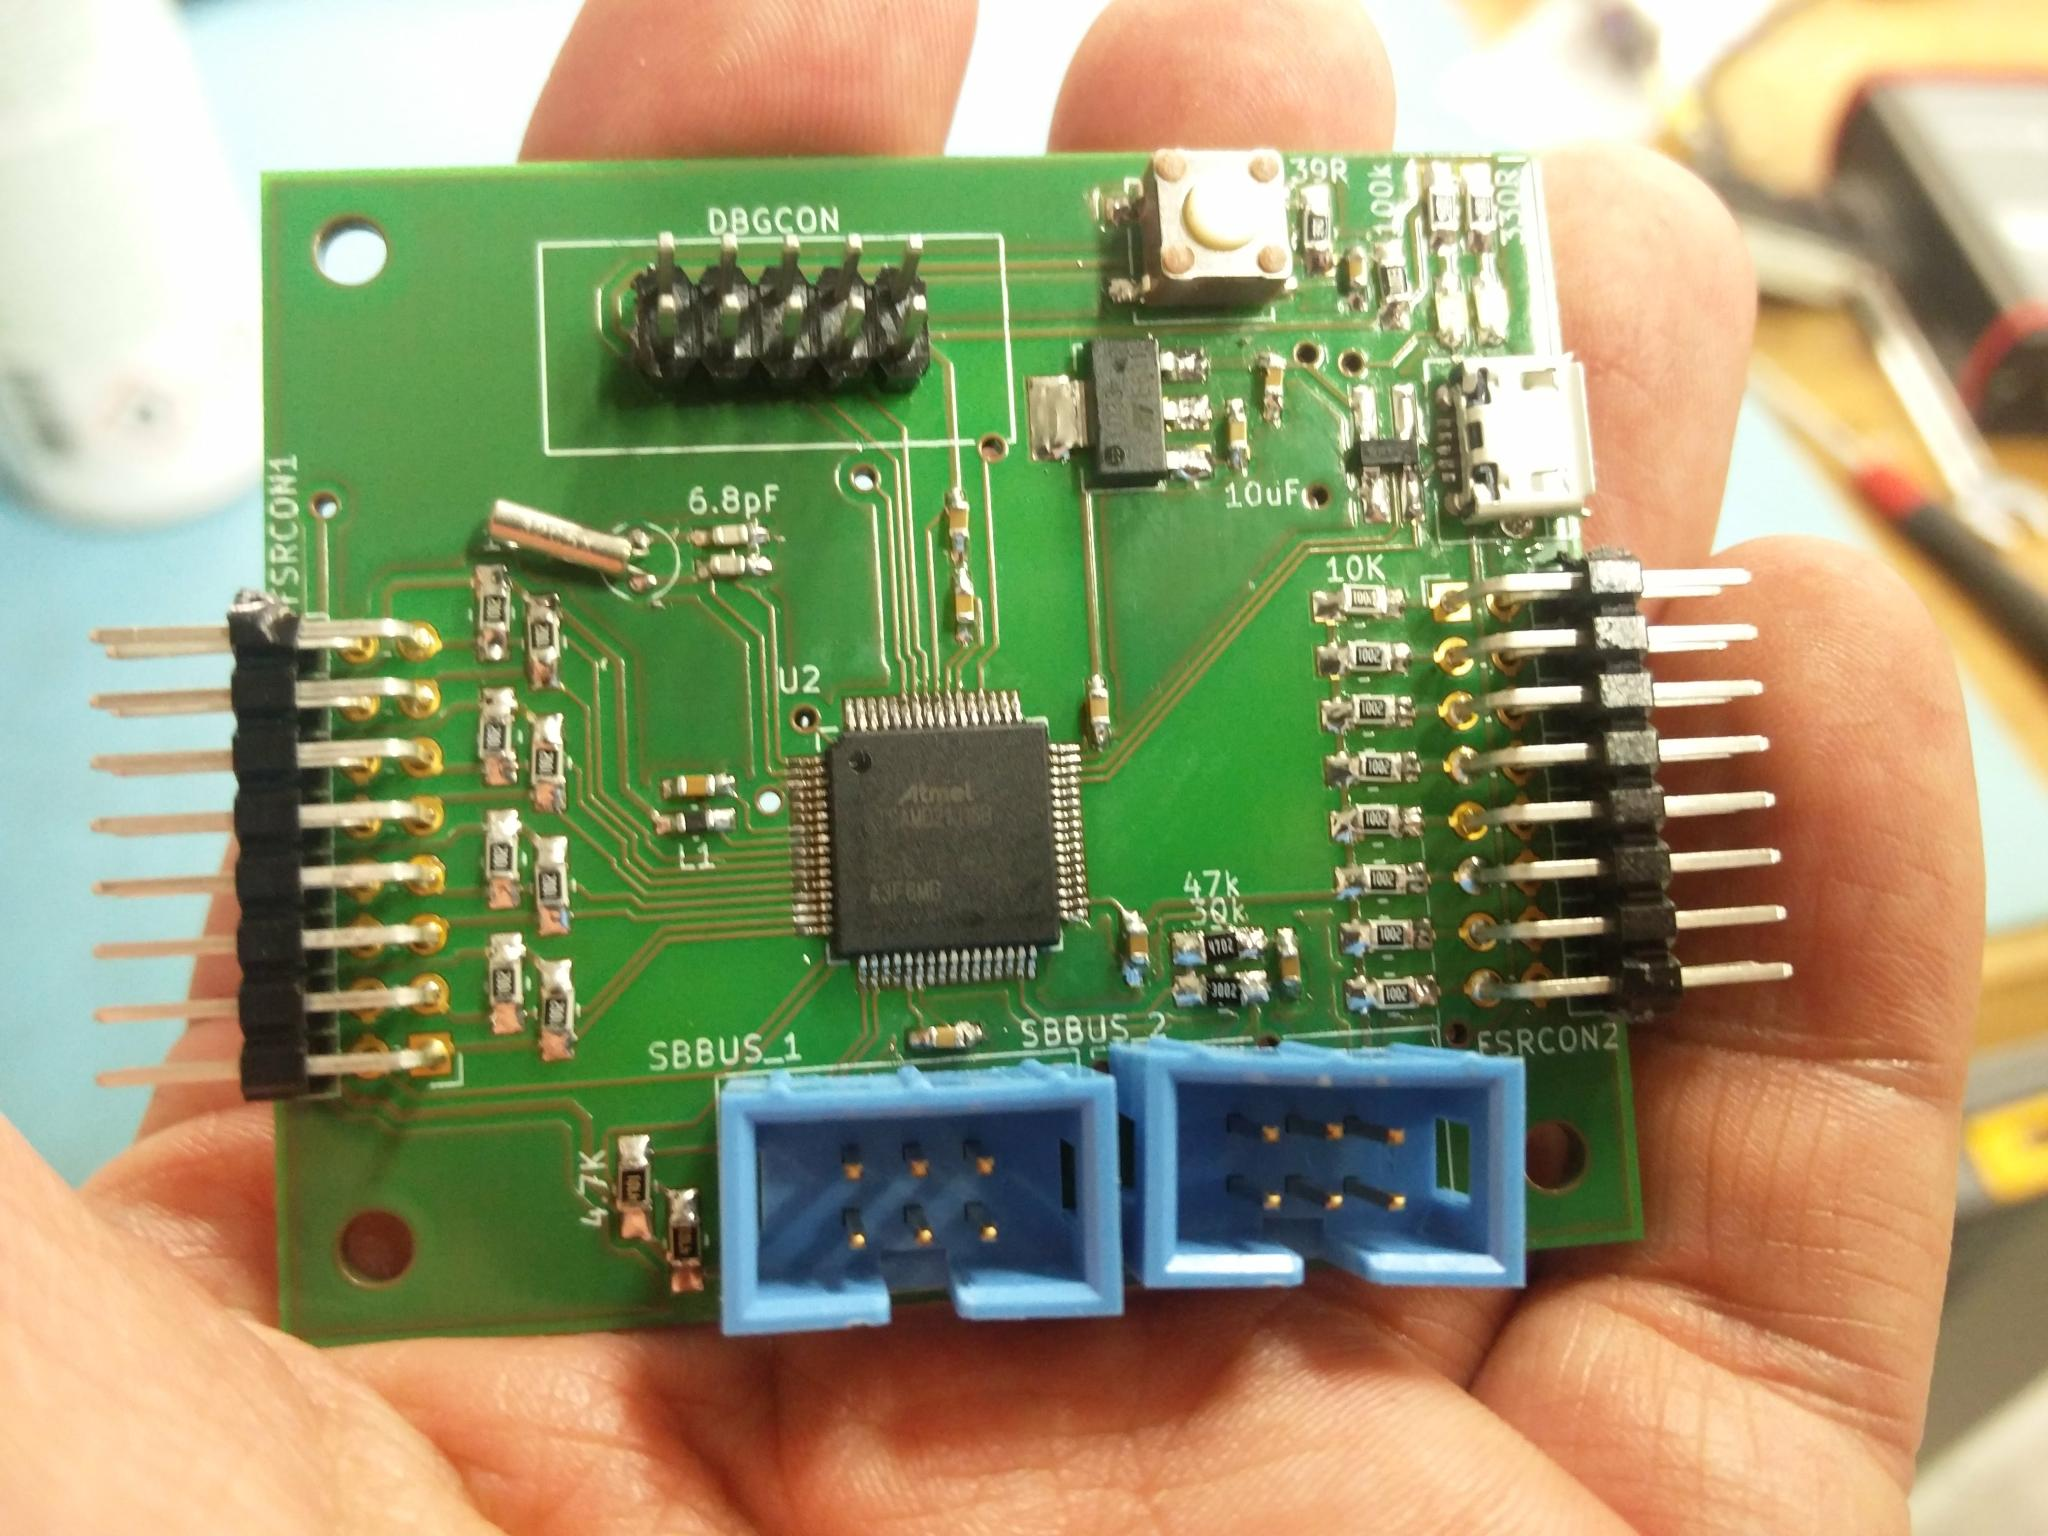
\includegraphics[width=0.45\linewidth]{2-pcb_production.jpg}
  \end{center}
  \caption{Fully populated node circuitboard.}
  \label{fig:pcb_production}
\end{figure}


\section{Development environment}

Because of the ARM architecture and Thumb2 instruction set, selected microcontroller supports multiple frameworks and development environments. One of most standardized and widely used frameworks is ARM mbed. It is compatible with almost all ARM microcontroller designs from vendors such as STMicroelectronics, NXP, Renesas, Nordic and Atmel\cite{mbed_devices}. Through abstraction it allows the same code to work on different devices. Depending on the selected device, application code is linked with platform specific libraries and a hex code output file is generated. This hex file can then be uploaded to the microcontroller using "drag and drop" or using \ac{SWD} interface\cite{SWD}. In case of this project, mbed framework was used through \href{http://platformio.org}{Platformio} open source ecosystem for \ac{IoT} development. This environment integrates in Microsoft's VSCode code editor and allows code compiling, upload and debugging along with other features such as intellisense code competition, unit testing and continuous integration. Although both mbed and Platformio support ATSAMD21J18 and Atmels Xplained Pro development board, they provide no support for ATSAMD21J16 variant of the microcontroller. This is why a new configuration for both had to be made.

First, a new board configuration was added to the Platformio configuration folder found in \code{\char`\~/.platformio/boards}. Then a \ac{JSON} structured file was created based upon Atmel Xplained Pro board file but maximum ram size and maximum size were changed because of the smaller \ac{RAM} and flash size. Then a support for a new processor had to be added to the mbed \ac{SDK}. First a new microcontroller and variant were declared an then microcontroller features were described in \code{.platformio/packages/framework-mbed/targets/targets.json}. and can be seen in Listing \ref{lst:mbed_config}. Then \ac{GPIO} port mapping of this chip variant is declared in \code{port\_api.c}. Next required change includes modification of load script. \ac{ROM} is set as rx memory form address 0x00000000 until address 0x00010000 while \ac{RAM} is of rwx type starting from 0x20000000 and with size of 0x2000. Stack size is defined to be 0x500. After these changes were introduced, \ac{BSP} can be generated using tool tox. After that, a board is visible in Platformio and programs can be compiled for it.

\begin{lstlisting}[language=json,firstnumber=1,caption={Description of mbed features implemented in ATSAMD21J16},label={lst:mbed_config}]
"SAMD21J16A": {
    "inherits": ["Target"],
    "core": "Cortex-M0+",
    "macros": ["__SAMD21J16A__", "I2C_MASTER_CALLBACK_MODE=true", "EXTINT_CALLBACK_MODE=true", "USART_CALLBACK_MODE=true", "TC_ASYNC=true"],
    "extra_labels": ["Atmel", "SAM_CortexM0P", "SAMD21"],
    "supported_toolchains": ["GCC_ARM", "ARM", "uARM"],
    "device_has": ["ANALOGIN", "ANALOGOUT", "I2C", "I2CSLAVE", "I2C_ASYNCH", "INTERRUPTIN", "PORTIN", "PORTINOUT", "PORTOUT", "PWMOUT", "RTC", "SERIAL", "SERIAL_ASYNCH", "SERIAL_FC", "SLEEP", "SPI", "SPISLAVE", "SPI_ASYNCH"],
    "release_versions": ["2"],
    "device_name": "ATSAMD21J16A"
}
\end{lstlisting}

After program has been compiled and linked for the specific microcontroller, the hex file needs to be uploaded to the microcontroller flash storage. Segger JLink programmer is used for this purpose. To automate the upload a custom script and configuration file were written and integrated into the Platformio. Debugger interface using OpenOCD was also setup so that microcontroller could be debugged from the same development environment. A preview found in Figure \textbf{TODO FIGURE} shows debugging user interface. 


\section{Software implementation}

\section{Installation and integration}

